\documentclass{report}

\usepackage{geometry}
\usepackage{graphicx}

\geometry{left=25mm, right=25mm, top=30mm, bottom=30mm}

\begin{document}
	
	{
		\pagenumbering{gobble}
		\centering
		--\\
		\hline
		\vskip3cm
		\Huge \texttt{RPi-R:R} \\
		\Large \texttt{Raspberry Pi-Rheometer: Reference}\\
		\vskip3cm
		\large For software version: 0.1.3\\
		\vfill
		\hline
		--\\
		\newpage
	}
	
	\tableofcontents
	
	\chapter{Overview}
	
		\pagenumbering{arabic}
		
		\section{Hardware}
			This section describes the main hardware that comprises the rheometer; the Taylor-couette cell, the bench, the scissor lift, etc. Most (i.e. all) of this was not of my design or choosing, it was set up by the department for a previous set of students, therefore I don't know the exact reasoning behind the choices, but I'll give it a go.
			
			The Taylor-Couette cell is composed of a hollow glass cylinder and a perspex inner cylinder. The inner cylinder is attached to the rotor of a DC motor. The outer cylinder is attached to a scissor lift. Fluid can be placed into the gap between the cylinders and sheared - this is roughly the whole rheometer. In addition, there are sensors and other electronics which allow the hardware to be controlled by a Raspberry Pi computer, discussed in the next section.
			
			The cell is based upon a heavy metal base, of unsure exact function. It is a nice way to organise the rheometer, it provides a stable base, and it protects the worktop, but a bare worktop would have been fine too. On this bench sits the scissor lift holding the fixed outer cylinder, as well as a clamp stand which holds the motor (and the inner cylinder).
			
			The motor is a 15V DC electric motor with a 1/16th reduction gear system attached. This motor can operate nominally with a voltage supply between 4.5V and 15V.
			
			There are some important geometries used in the rheometry calculation; the diameters of the inner and outer cylinders. These are summarised in Table \ref{tablegeoms}.
			
			\begin{table}
				\centering
				\caption{Summary of Hardware Geometries}
				\label{tablegeoms}
				\begin{tabular}{| c | c | c |}
					\hline
					\textbf{Dimension} & \textbf{Symbol} & \textbf{Value} \\ \hline
					Inner cylinder diameter & $\rm D_{IC}$ & 0.035 m \\ \hline
					Outer cylinder diameter (outer) & $\rm D_{OCo}$ & 0.044 m \\ \hline
					Outer cylinder diameter (inner) & $\rm D_{OCi}$ & 0.039 m \\ \hline
				\end{tabular}
			\end{table}
			
			\subsection*{Known Issues}
				\textbf{Assumption:} Couette flow in between the cylinders. \textbf{Strengths:} the cylinders have a small gap, and can be easily adjusted to minimise errors in centring. \textbf{Weaknesses:} both the inner and outer cylinders have small imperfections which could affect the flow in the cell. The glass outer cylinder is non uniform --- to be expected with glass objects. Also, the inner cylinder is slightly off centre --- slightly.
				
				\textbf{Assumption:} motor gear system will not greatly affect the system, or it will but in a way that can be accounted for in calibrations. \textbf{Strengths:} this should be true for any well maintained gear system. Gears only transfer movement and should not present any resistance that is not easily accounted for. \textbf{Weaknesses:} the gear system/motor sometimes acts oddle --- making strange sounds and appearing to slow despite no changes to load or to power supply. This was remedied (hopefully) by applying WD40 to the gear system.
			
		\section{Electronics}
		
			The electronics of the RPi-R consist of two sections: motor supply voltage control, and sensor readings. Both based on breadboard (at the moment --- the prototype is subject to change, so nothing too permanent). The former consists of a digital potentiometer (a digitally programmable variable resistor) which alters the voltage going into an operational amplifier (very useful IC) which in this case is used to boost the voltage 2.1 times. The current is then boosted by a transistor roughly 200 times to around 2A. The sensors are all fed into an Analogue to Digital Converter (ADC).
			
			The electronic system is connected to the Raspberry Pi using serial data transfer. Serial, as opposed to parallel, sends data as bits one after the other down one or more lines to as regulated by a clock signal. The SPI (Serial Peripheral Interface) protocol is the main serial interface used. One wire (1-Wire) is also used, but only for the temperature sensor.
			
			The voltage regulation consists of a digital potentiometer which is controlled by the RPi via SPI. A signal (7-bit number, 0-127) is sent from the Pi, and represents the position of the wiper of the potentiometer and thus the resistance and the voltage on the wiper. This wiper voltage is amplified by an operational amplifier (in non-inverting operational mode) such that the voltage is able to be swept between around 2.4 volts up to 10.8 volts. This amplified voltage is passed through the base of a transistor which is used to boost its current up to a reasonably large 2A available. This transistor is therefore having to pass a high current and high voltage - it understandably therefore heats up a great deal\footnote{Before the heatsink was attached, the transistor melted a section out of the breadboard. Then, after I attached wires to remove it from other components, it melted the wires. The transistor can get \textbf{very} hot.}. This was dealt with by adding a heatsink\footnote{Which can also get quite hot. I managed to burn a lovely pattern onto my thumb.} to the transistor. The heatsink may not be sufficient, a fan or larger heatsink may be necessary.
			
			The ADC is an 8 channel, 10-bit analogue to digital converter. It compares the voltage level at each of its 8 input channels to a voltage reference (3.3V --- from the Raspberry Pi): this value is sent, via SPI, to the RPi as a number between 0 and 1023 (a 10-bit number).
			
		
		\section{Software}
		
		\section{Summary}
		
			Presented here are lists of every component used to construct the RPi-R, along with links to datasheets if possible, as well as the circuit diagrams and photographs of the actual layout.
	
	\chapter{Usage}
	
		\section{Using the rheometer script}
		
		The \texttt{rheometer.py} script should be run from the command line in your favourite terminal emulator. Normally, you should only need to run the script alone (no arguments), however there are two recognised:
		\begin{verbatim}
			python rheometer.py [-r|-c]
			
			-c: complex calculation mode
			-r: "raw" mode
		\end{verbatim}
		``Raw'' mode does not catch errors as they occur, instead throws the excpetions to the user. Use this flag if the rheometer is acting up. Complex calculation mode is, as the name suggests, a more complex way of calculating the rheometry of the test fluid. However, this mode has not been finished and has proved very troublesome. Hence, simple mode is used by default.
		
		Once the rheometry script has started up, you will be greeted by the main menu. From here you can choose what you want to do. Use up and down the arrow keys to navigate the options, and the enter key to select. Figure \ref{figmenumain} is a screenshot of the main menu. 
		
		\begin{figure}
			\centering
			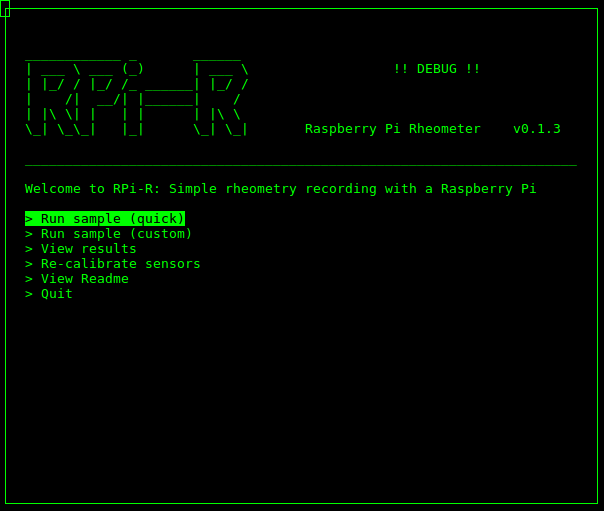
\includegraphics[width=.8\textwidth]{./../graphics/figmenumain.png}
			\caption{Main Menu}
			\label{figmenumain}
		\end{figure}
		
		The menu has 5 options. The first two ("Run sample (quick)", "Run sample (custom") run the data logger and control the voltage supply to the motor. The information from these tests are saved in comma separated value (.csv) files, (in the "logs" folder). These files can be automatically read, the data extracted, and the results calculated using the \texttt{"docs/gen\_rep.py"} script. Alternatively, the .csv log files can be opened in your favourite spreadsheet program (MS Office Excel, Libre Office Calc, \&c). The quick test uses middling preset options (these can be altered in the script). The custom test allows you to set the run parameters before starting. There are two parameters for a run: run length, and strain rate. The run length is given in seconds. The strain rate, in inverse seconds, can be defined as a function of time (if you wish), or just give a constant. An optional parameter of the test run is a string informational tag attached to the log to identify what physical parameters have been set (e.g. fluid concentration, volume, temperature \&c). Once the run has finished, the save location of the log will appear on screen.
		
		The third menu option ("View results") does nothing at the moment. Neither does the fourth option. The fifth, shows a vague summary of what the rheometer does. And finally, "Quit" exits the program.
	
	\chapter{}
	
	\chapter{Forte, For}

	

\end{document}